\documentclass[a4paper,11pt,onecolumn]{report}
\usepackage[T1]{fontenc} % Fontes T1
\usepackage[utf8]{inputenc} % Input UTF8
\usepackage[backend=biber, style=ieee]{biblatex} % para usar bibliografia
\usepackage{csquotes}
\usepackage[portuguese]{babel} %Usar língua inglesa
\usepackage{blindtext} % Gerar texto automáticamente
\usepackage[printonlyused]{acronym}
\usepackage{hyperref} % para autoref
\usepackage{graphicx}
\usepackage{minted}
\usepackage{indentfirst}
\usepackage{array}
\newcolumntype{L}[1]{>{\raggedright\let\newline\\\arraybackslash\hspace{0pt}}m{#1}}
\newcolumntype{C}[1]{>{\centering\let\newline\\\arraybackslash\hspace{0pt}}m{#1}}
\newcolumntype{R}[1]{>{\raggedleft\let\newline\\\arraybackslash\hspace{0pt}}m{#1}}


\bibliography{bibliografia}
\addbibresource{bibliografia.bib}


\begin{document}
%%
% Definições
%
\def\titulo{Temporizador de Reação}
\def\data{06/05/2015}
\def\autores{Pedro Martins, Pedro Santos}
\def\autorescontactos{pbmartins@ua.pt, pedroamaralsantos@ua.pt}
\def\versao{1}
\def\departamento{Departamento de Eletrónica Telecomunicações e Informática}
\def\empresa{Universidade de Aveiro}
\def\logotipo{ua.pdf}
%
%% CAPA %%
%
\begin{titlepage}

\begin{center}
%
\vspace*{50mm}
%
{\Huge \titulo}\\ 
%
\vspace{10mm}
%
{\Large \empresa}\\
%
\vspace{10mm}
%
{\LARGE \autores}\\ 
%
%
\vspace{30mm}
%
\begin{figure}[h]
\center
\includegraphics{\logotipo}
\end{figure}
%
\vspace{30mm}
\end{center}
%
\begin{flushright}
\versao
\end{flushright}
\end{titlepage}

%
%
%%  Página de Título %%
%
%
\title{%
{\Huge\textbf{\titulo}}\\
{\Large \departamento\\ \empresa}
}
%
\author{%
    \autores \\
    \autorescontactos
}
%
\date{\data}
%
\maketitle

%%%%%%%%%%%%%%%%%%%%%%%%%%%%%%%%%%%%%%%%%%%
% RESUMO
%
%
\pagenumbering{roman}

\tableofcontents


%%%%%%%%%%%%%%%%%%%%%%%%%%%%%%%
\clearpage
\pagenumbering{arabic}

%%%%%%%%%%%%%%%%%%%%%%%%%%%%%%%%
\chapter{Introdução}
\label{chap.introducao}

Foi-nos proposto a criação de um mini-projeto na disciplina de Laboratórios de Sistemas Digitais, utilizando uma \ac{fpga} e \ac{vhdl}. Foi determinado pelo grupo que seria implementado um simples temporizador de reação utilizando máquinas de estados e diversos outros recursos.

\chapter{Análise}
\label{chap.analise}

\section{Especificações do Sistema}\ac{fpga}
O mini-projeto em análise consiste na implementação de um temporizador de reação. A ideia pode traduzir-se como, depois de aceso um LED, medir o tempo que o utilizador demora a carregar num botão, registando o tempo entre ambos. Apenas serão aceites dois botões, um para fazer \textit{Reset} ao sistema em qualquer ponto do seu funcionamento, e outro para o início do jogo e que também servirá como o botão que o utilizador tem de pressionar para calcular o tempo de reação.

Assim que o utilizador carrega inicialmente no botão de iniciar o jogo, é gerado um número aleatório entre 5 e 60 (e validado), que será o tempo, em segundos, que demorará o LED a acender desde que se iniciou o jogo. De seguida, é utilizado um "semáforo de partida", onde a cada segundo, 3 LED vermelhos se apagam até que começa a contar o tempo até que o LED indicador se acenda.

Se o utilizador carregar no botão de jogar antes de o LED acender, é impresso nos ecrãs hexadecimais uma mensagem de erro. Caso o utilizador apenas clique no botão depois de aceso, é imprimido no ecrãs hexadecimais o tempo percorrido desde que o LED acendeu até o mesmo carregar no botão. A \ac{fpga} manter-se-á neste estado até que se volte a reiniciar o jogo, isto é, clicar no botão de \textit{Reset}, onde todos os painéis hexadecimais e todos os LED serão apagados.

\pagebreak

\section{Arquitetura}
A \autoref{figblocos} apresenta uma arquitetura do sistema em geral.

%figura 1%
\begin{figure}[h]
\centerline{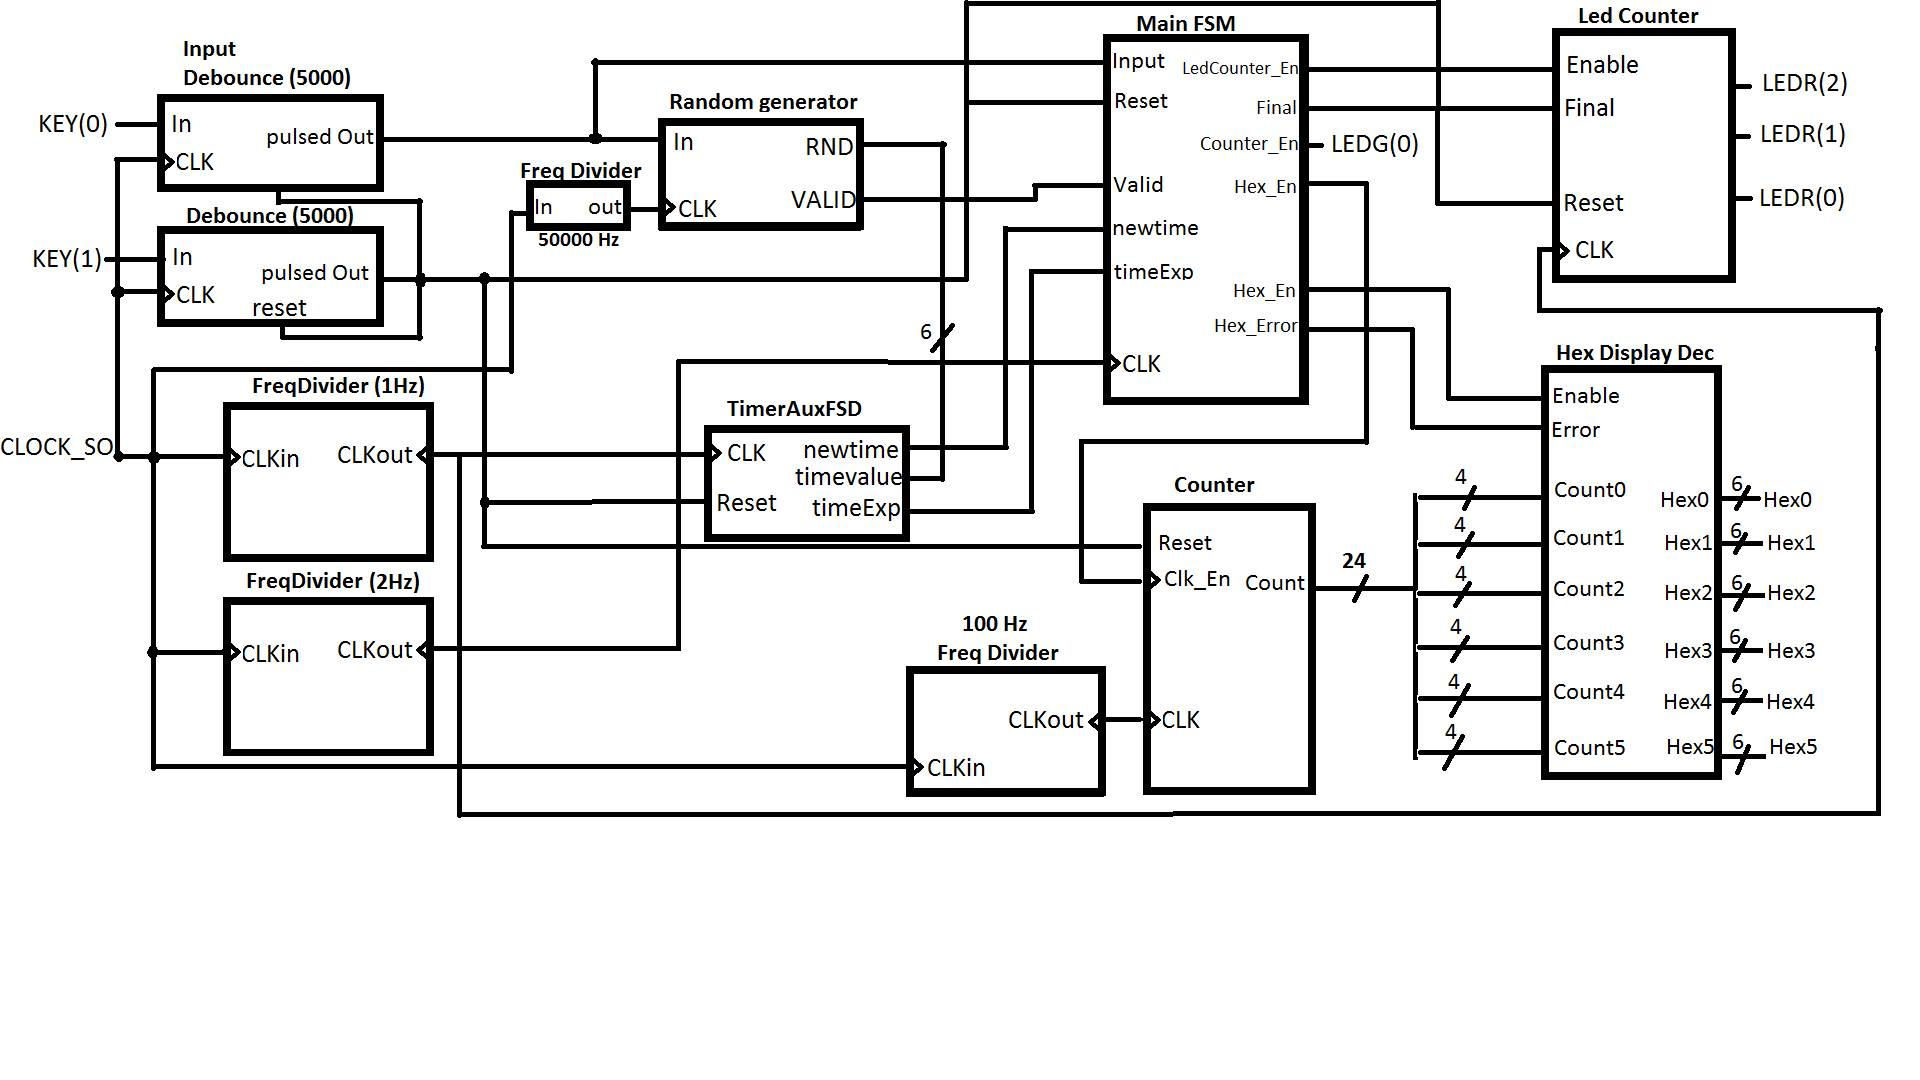
\includegraphics[scale=0.25]{Images/BlockDiagram}}
\caption{Arquitetura do temporizador de reação.}
\label{figblocos}
\end{figure}

\pagebreak

Para além das máquinas de estado, existem outros blocos que são constituídos por vários sub-blocos. Apresentam-se o seguintes diagramas:

%figura 2%
\begin{figure}[h]
\centerline{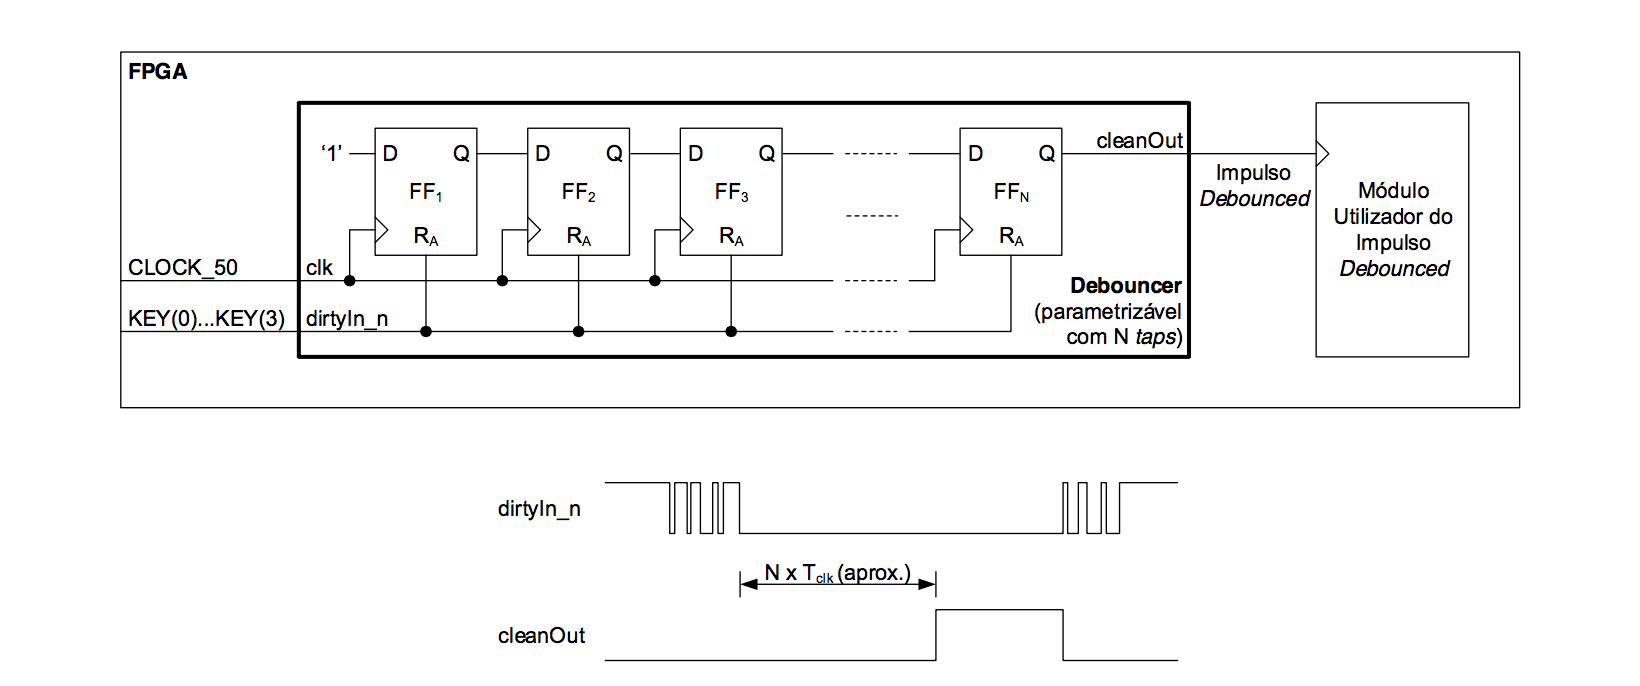
\includegraphics[scale=0.3]{Images/debouncerBlock}}
\caption{Arquitetura do \textit{debouncer}, desenvolvido pelos professores da disciplina.}
\label{figdebounce}
\end{figure}

%figura 3%
\begin{figure}[h]
\centerline{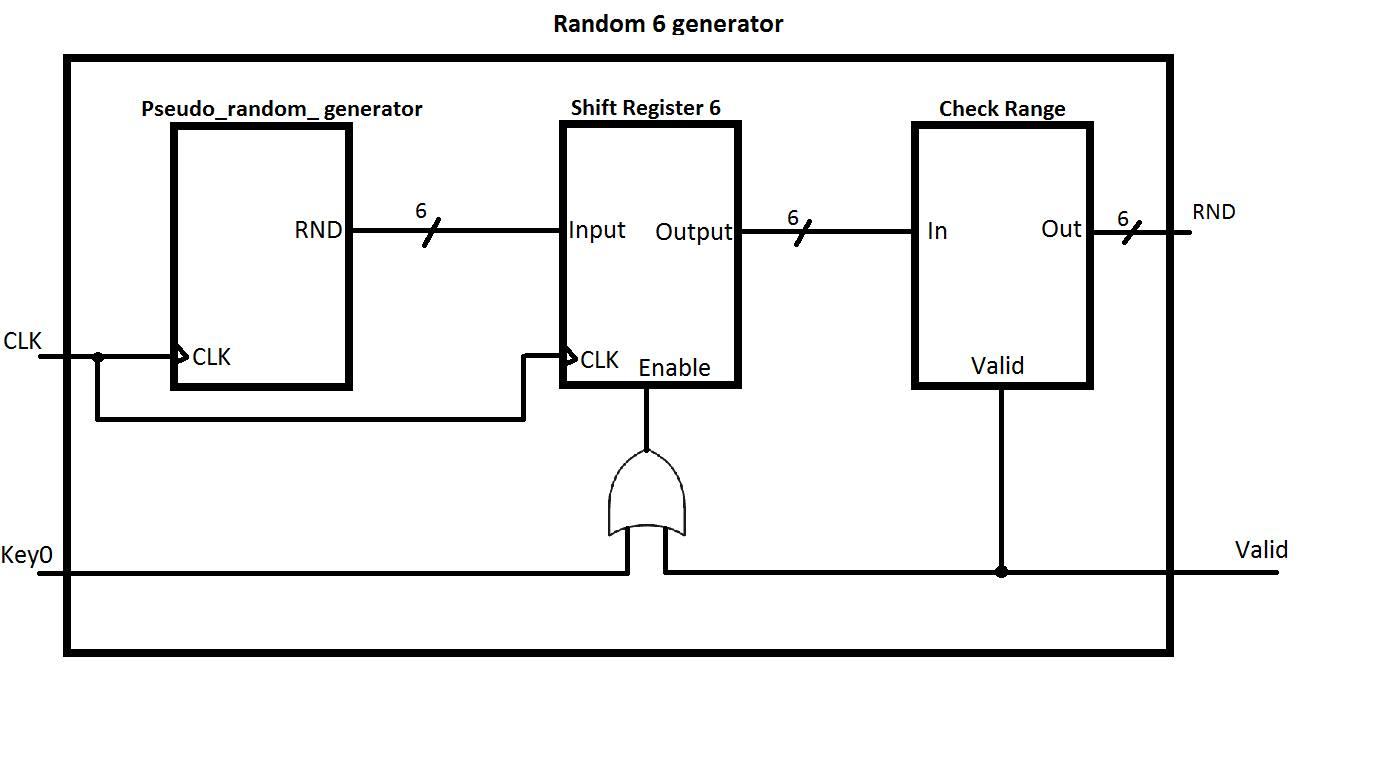
\includegraphics[scale=0.3]{Images/RandomGenerator}}
\caption{Arquitetura do gerador de números aleatórios.}
\label{figrndgenerator}
\end{figure}

\pagebreak

Por outro lado, são apresentados os diagramas de estados das máquinas de estados \textit{Main FSM}, \textit{Timer Aux FSM} e \textit{LEDCounter FSM}.

%figura 5%
\begin{figure}[h]
\centerline{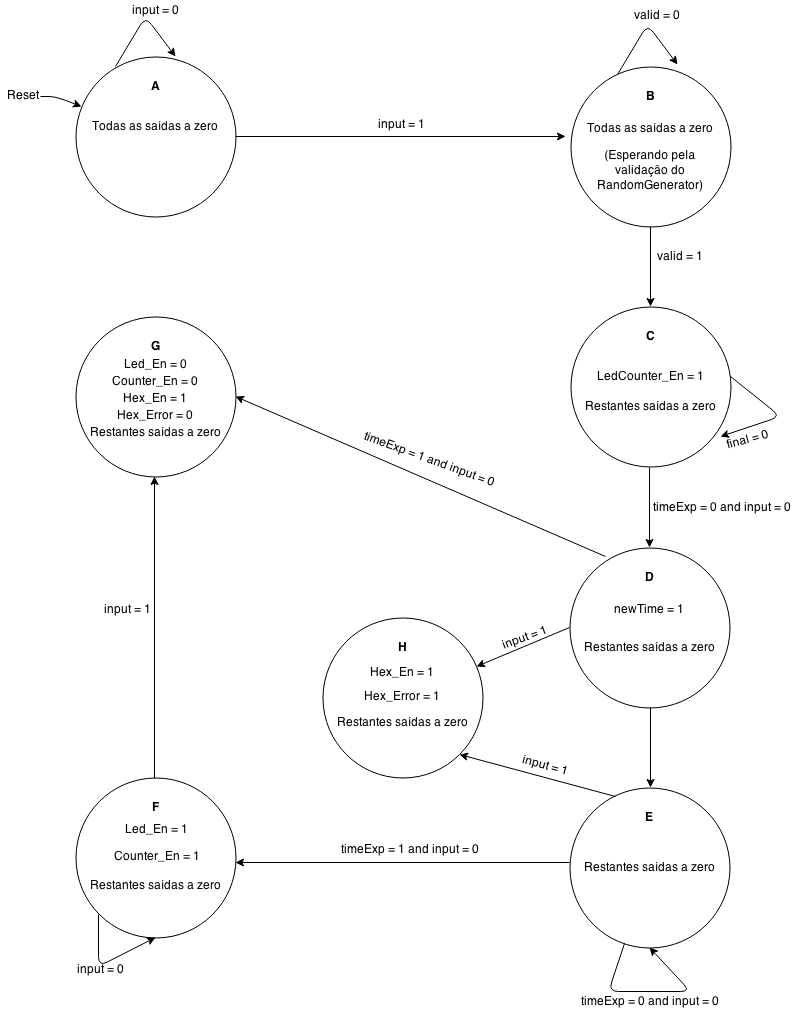
\includegraphics[scale=0.4]{Images/MainFSMDiagram}}
\caption{Diagrama de estados da \textit{Main FSM}.}
\label{figmainfsm}
\end{figure}

\pagebreak

%figura 6%
\begin{figure}[h]
\centerline{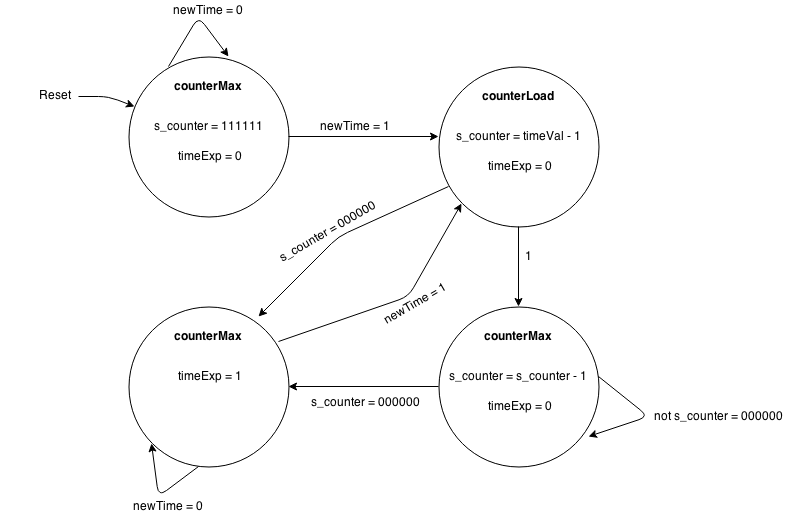
\includegraphics[scale=0.33]{Images/TimerAuxFSMDiagram}}
\caption{Diagrama de estados da \textit{Timer Aux FSM}.}
\label{figtimerfsm}
\end{figure}

%figura 7%
\begin{figure}[h]
\centerline{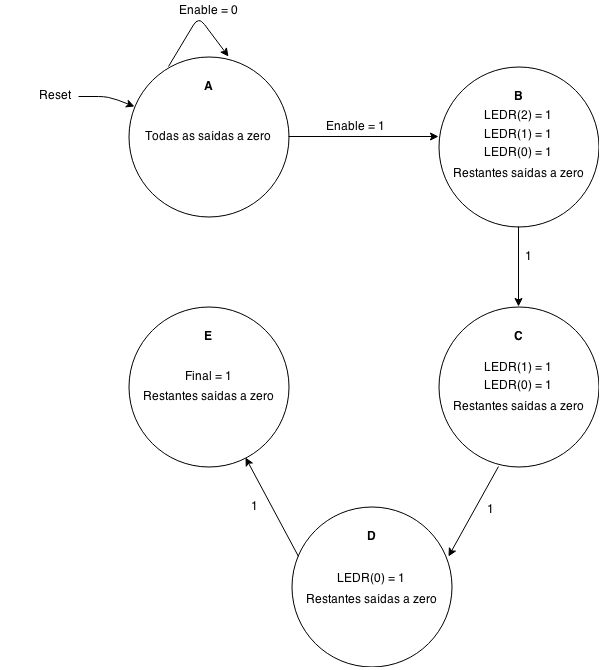
\includegraphics[scale=0.30]{Images/CounterLEDFSMDiagram}}
\caption{Arquitetura do \textit{LEDCounterFSM}.}
\label{figledcounterfsm}
\end{figure}

\pagebreak

\section{Abordagem Faseada do Desenvolvimento}
Como se pode verificar na \autoref{figblocos}, o "núcleo" de funcionamento do temporizador de reação assenta na parceria entre as duas máquinas de estados, a \textit{Main FSM} e a \textit{Timer Aux FSM}. Depois de construídas estas duas máquinas, serão também desenvolvidos os blocos do contador do tempo de reação, assim como o descodificador de binário para hexadecimal.

Primeiramente, serão implementados os \textit{debouncers} nas entradas do circuito (KEY(0) e KEY(1)), para evitar oscilações quando os botões são pressionados.

Numa fase inicial, será ignorado o "semáforo de partida" e o gerador de números aleatórios. Logo, a entrada \textit{timeVal} na máquina de estados \textit{Timer Aux FSM} terá o valor 10 (10 segundos, isto é, 001010 em binário), enquanto que, em relação à \textit{Main FSM}, a saída \textit{LEDCounter\_En} será ignorada e a entrada \textit{Final} terá sempre o valor 1 ("salta" o "semáforo"). Serão também utilizados vários divisores de frequência para que os impulsos de relógio sejam a cada 1 segundo (\textit{Timer Aux FSM}), e a cada centésimo de segundo (\textit{ReactionTimeCounter}).

Assim que realizados e validados os testes sobre a entidade acima descrita, adicionar-se-ão os restantes blocos, o \textit{LEDCounter FSM} ("semáforo de partida"), ao qual será ligado um divisor de frequência de 1Hz (impulsos a cada segundo) e o \textit{RandomGenerator}, ao qual será ligado um divisor de frequência de 50000 Hz.

Por fim, serão executados novos testes para validar o funcionamento da entidade global do temporizador de reação.

\section{Divisão de Tarefas}
Em seguida, apresenta-se a divisão de tarefas do projeto e quais os blocos que cada elemento deve construir.

Pedro Martins:
\begin{itemize}
\item \textit{Main FSM};
\item \textit{Time Aux FSM};
\item \textit{ReactionTimeCounter};
\item \textit{Testbench} - unidade de testes.
\end{itemize}

\pagebreak

Pedro Santos:
\begin{itemize}
\item \textit{Debouncer};
\item \textit{FreqDivider};
\item \textit{LEDCounter FSM};
\item \textit{HexDisplaysDecoder};
\item \textit{Testbench} - unidade de testes.
\end{itemize}

\section{Manual de Instruções}
Para medir o seu tempo de reação, deve seguir os seguintes passos:
\begin{itemize}
\item Certificar-se que a \ac{fpga} está corretamente ligada e programada;
\item Pressionar o botão KEY(0), para iniciar o jogo;
\item Aguardar que os três LED vermelhos se apaguem;
\item Clicar no botão KEY(0) logo depois de o LED verde se acender;
\item Será impresso no ecrã hexadecimal o seu tempo de reação;
\item Para reiniciar o jogo, tem de clicar no botão KEY(1) e repetir todos os passos acima descritos.
\end{itemize}


\chapter{Conclusões}
\label{chap.conclusao}
Em suma, depois de estabelecida a arquitetura do sistema, os vários diagramas de estados e a divisão de tarefas, é possível passar à prática e programar o circuito.


%%%%%%%%%%%%%%%%%%%%%%%%%%%%%%%%%
\chapter*{Acrónimos}
\begin{acronym}
\acro{ua}[UA]{Universidade de Aveiro}
\acro{miect}[MIECT]{Mestrado Integrado em Engenharia de Computadores e Telemática}
\acro{fpga}[FPGA]{Field-Programmable Gate Array}
\acro{vhdl}[VHDL]{Very high speed integrated circuit Hardware Description Language}

\end{acronym}


%%%%%%%%%%%%%%%%%%%%%%%%%%%%%%%%%

\end{document}
